%------------------------------------------------------------------------------
% CV in Latex
% Author : Huanfa Chen
% Inspired by and adapted from: https://github.com/sb2nov/resume and Jake's Resume on Overleaf
% Most recently updated version may be found at https://github.com/huanfachen/Huanfa_CV 
% License : MIT
%------------------------------------------------------------------------------

\documentclass[A4,11pt]{article}
%\documentclass[letterpaper,11pt]{article} %For use in US
\usepackage{latexsym}
\usepackage[empty]{fullpage}
\usepackage{titlesec}
\usepackage{marvosym}
\usepackage[usenames,dvipsnames]{color}
\usepackage{verbatim}
\usepackage{enumitem}
\usepackage[hidelinks]{hyperref}
\usepackage[english]{babel}
\usepackage{tabularx}
\usepackage{tikz}

\input{glyphtounicode}

\begin{comment}
I am by no means a professional when it comes to the CV's/resumes, I have
received various trainings on how to write a CV and resume from my high 
school, as well as the Austin College and University of Eastern Finland's
career counseling departments. As I intend to share my CV as a template, I 
feel that it is my responsibility to provide explanations of my work.
\end{comment}

%% Set up citations and bibliography
\usepackage{bibunits}
\usepackage[sort&compress,super]{natbib}
\defaultbibliographystyle{apsrev4-2}
\setcitestyle{comma}
\setlength{\bibsep}{0pt}
\renewcommand{\bibnumfmt}[1]{\ \ \ #1.}
\renewcommand\refname{\vspace{-7mm}}
% \renewcommand\refname{}
\renewcommand{\bibsection}{}

%% This allows us to start a bibliography with arbitrary number
\usepackage{etoolbox}
\patchcmd{\thebibliography}{\section*{\refname}}{}{}{}
\makeatletter
\newcommand*{\newbibstartnumber}[1]{%
  \apptocmd{\thebibliography}{%
    \global\c@NAT@ctr #1\relax
    \addtocounter{NAT@ctr}{-1}%
  }{}{}%
}
\makeatother

%% Set up footer
\usepackage{fancyhdr}
\usepackage{lastpage}
\usepackage[nodayofweek,level]{datetime}
\fancypagestyle{CVfooter}
{
 \lhead{}
 \chead{}
 \rhead{}
 \lfoot{\small{Huanfa Chen}}
 \cfoot{\small{Last update: \today}}
 \rfoot{\small{\thepage/\pageref{LastPage}}}
 \renewcommand{\headrulewidth}{0.0pt}
 \renewcommand{\footrulewidth}{0.5pt}
}

%-----FONT OPTIONS-------------------------------------------------------------
\begin{comment}
The font of the document will impact not just how readable it is, but how it is
perceived. In the "The Craft of Scientific Writing" by Michael Alley, shares a
common fonts for publication as well as their use. I have chosen to use
Palatino for its legibility, some others are given below. There is far too much
about typography to discus here. Note: serif fonts have short projecting
strokes, sans-serif fonts are sans (without) these strokes.
\end{comment}


% serif
 \usepackage{palatino}
% \usepackage{times} %This is the default as well
% \usepackage{charter}

% sans-serif
% \usepackage{helvet}
% \usepackage[sfdefault]{noto-sans}
% \usepackage[default]{sourcesanspro}

%-----PAGE SETUP---------------------------------------------------------------
% https://en.wikibooks.org/wiki/LaTeX/Page_Layout

% Adjust margins
% \usepackage[left=1.0in, right=1.0in, top=1.0in, bottom=1.0in]{geometry} % margins
% \usepackage{setspace}
% \singlespacing % No more than 6 lines of text per inch
\addtolength{\oddsidemargin}{-1cm}
\addtolength{\evensidemargin}{-1cm}
\addtolength{\textwidth}{2cm}
\addtolength{\topmargin}{-1cm}
\addtolength{\textheight}{2cm}
\addtolength{\footskip}{20pt}
% note the defatult footskip = 30 pt. Increasing the footskip will lower the position of the footer to the page bottom

% %% Page and text formatting
% \usepackage[left=1.0in, right=1.0in, top=1.0in, bottom=1.0in]{geometry} % margins
% \usepackage{setspace}
% \singlespacing % No more than 6 lines of text per inch
% \usepackage{amsmath, amsfonts}
% \usepackage[T1]{fontenc}
% \usepackage{times}

% Margins for US Letter size
%\addtolength{\oddsidemargin}{-0.5in}
%\addtolength{\evensidemargin}{-0.5in}
%\addtolength{\textwidth}{1in}
%\addtolength{\topmargin}{-.5in}
%\addtolength{\textheight}{1.0in}

\urlstyle{same}

\raggedbottom
\raggedright
\setlength{\tabcolsep}{0cm}

% Sections formatting
\titleformat{\section}{
  \vspace{-4pt}\scshape\raggedright\large
}{}{0em}{}[\color{black}\titlerule \vspace{-5pt}]

% Ensure that .pdf is machine readable/ATS parsable
\pdfgentounicode=1

%-----CUSTOM COMMANDS FOR FORMATTING SECTIONS----------------------------------
\newcommand{\CVItem}[1]{
  \item\small{
    {#1 \vspace{-2pt}}
  }
}

\newcommand{\MScStduentItem}[4]{
  \item #1 (#2, #3)
   \begin{itemize}
    \item[$\textendash$] \ #4
   \end{itemize}
}

\newcommand{\CVSubheading}[4]{
  \vspace{-2pt}\item
    \begin{tabular*}{0.97\textwidth}[t]{l@{\extracolsep{\fill}}r}
      \textbf{#1} & #2 \\
      \small#3 & \small #4 \\
    \end{tabular*}\vspace{-7pt}
}

\newcommand{\CVSubheadingSimple}[2]{
  \vspace{-2pt}\item
    \begin{tabular*}{0.97\textwidth}[t]{l@{\extracolsep{\fill}}r}
      \textbf{#1} & #2 \\
    \end{tabular*}\vspace{-7pt}
}

\newcommand{\CVSubSubheading}[2]{
    \item
    \begin{tabular*}{0.97\textwidth}{l@{\extracolsep{\fill}}r}
      \text{\small#1} & \text{\small #2} \\
    \end{tabular*}\vspace{-7pt}
}

\newcommand{\CVSubItem}[1]{\CVItem{#1}\vspace{-4pt}}

\renewcommand\labelitemii{$\vcenter{\hbox{\tiny$\bullet$}}$}

\newcommand{\CVSubHeadingListStart}{\begin{itemize}[leftmargin=0.5cm, label={}]}
% \newcommand{\resumeSubHeadingListStart}{\begin{itemize}[leftmargin=0.15in, label={}]} % Uncomment for US
\newcommand{\CVSubHeadingListEnd}{\end{itemize}}
\newcommand{\CVItemListStart}{\begin{itemize}}
\newcommand{\CVItemListEnd}{\end{itemize}\vspace{-5pt}}

%------------------------------------------------------------------------------
% CV STARTS HERE  %
%------------------------------------------------------------------------------
\begin{document}
\pagestyle{CVfooter}

%-----HEADING------------------------------------------------------------------
\begin{comment}
Avoid using photos in academic CV
\end{comment}

% \begin{minipage}[c]{0.05\textwidth}
% \-\
% \end{minipage}
% \begin{minipage}[c]{0.2\textwidth}
% \begin{tikzpicture}
%     \clip (0,0) circle (1.75cm);
%     \node at (0,-.7) {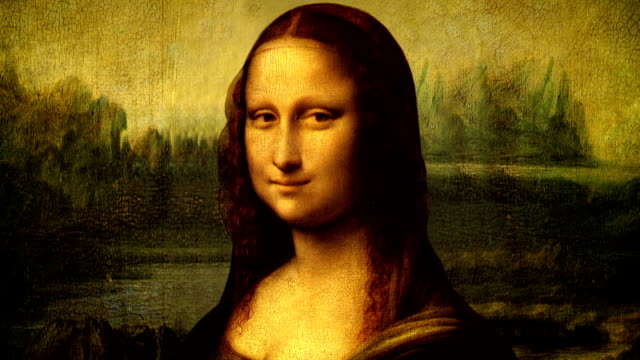
\includegraphics[width = 9cm]{portrait}}; 
%     % if necessary the picture may be moved by changing the at (coordinates)
%     % width defines the 'zoom' of the picture
% \end{tikzpicture}
% \hfill\vline\hfill
% \end{minipage}
% \begin{minipage}[c]{0.4\textwidth}
%     \textbf{\Huge \scshape{Charles Rambo}} \\ \vspace{1pt} 
%     % \scshape sets small capital letters, remove if desired
%     \small{+1 123-456-7890} \\
%     \href{mailto:you@provider.com}{\underline{you@provider.com}}\\
%     % Be sure to use a professional *personal* email address
%     \href{https://www.linkedin.com/in/charles-rambo/}{\underline{linkedin.com/in/charles-rambo}} \\
%     % you should adjust you linked in profile name to be professional and recognizable
%     \href{https://github.com/fizixmastr}{\underline{github.com/fizixmastr}}
% \end{minipage}

% Without picture
\begin{center}
    \textbf{\Huge \scshape Huanfa Chen} \\ \vspace{1pt} %\scshape sets small capital letters, remove if desired
    % \small +1 123-456-7890 $|$ 
    \href{mailto:huanfa.chen@ucl.ac.uk}{\underline{huanfa.chen@ucl.ac.uk}} $|$
    \href{huanfachen.github.io}{\underline{https://huanfachen.github.io/}} $|$\\
    % Be sure to use a professional *personal* email address
    \href{linkedin.com/in/huanfa-chen}{\underline{linkedin.com/in/huanfa-chen}} $|$
    % you should adjust you linked in profile name to be professional and recognizable
    \href{https://github.com/huanfachen}{\underline{github.com/huanfachen}}
\end{center}


\begin{comment}
This CV was written for specifically for positions I was applying for in
academia, and then modified to be a template.

A standard CV is about two pages long where as a resume in the US is one page.
sections can be added and removed here with this in mind. In my experience, 
education, and applicable work experience and skills are the most import things
to include on a resume. For a CV the Europass CV suggests the categories: Work
Experience, Education and Training, Language Skills, Digital Skills,
Communication and Interpersonal Skills, Conferences and Seminars, Creative Works
Driver's License, Hobbies and Interests, Honors and Awards, Management and
Leadership Skills, Networks and Memberships, Organizational Skills, Projects,
Publications, Recommendations, Social and Political Activities, Volunteering.

Your goal is to convey a who, what , when, where, why for every item you share. 
The who is obviously you, but I believe the rest should be done in that order.
For example below. An employer cares most about the degree held and typically 
less about the institution or where it is located (This is still good 
information though). Whatever order you choose be consistent throughout.
\end{comment}

%-----EDUCATION----------------------------------------------------------------
\section{Education}
  \CVSubHeadingListStart
%    \CVSubheading % Example
%      {Degree Achieved}{Years of Study}
%      {Institution of Study}{Where it is located}
    \CVSubheading
      {{Doctor of Philosophy $|$ \emph{\small{Geographic Information Science}}}}{Sep 2014 -- Feb 2019}
      {University College London}{London, UK}
    \CVSubheading
      {{Master of Science $|$ \emph{\small{Geographic Information Systems and Cartography}}}}{Sep 2011 -- July 2014}
      {Peking University}{Beijing, China}
    \CVSubheading
      {{Bachelor of Science $|$ \emph{\small{Chemistry}}}}{Sep 2007 -- July 2011}
      {Peking University}{Beijing, China} 
  \CVSubHeadingListEnd

%-----WORK EXPERIENCE----------------------------------------------------------
\begin{comment}
try to briefly explain what you did and why it is relevant to the position you
are seeking
\end{comment}

\section{Work Experience}
  \CVSubHeadingListStart
%    \CVSubheading %Example
%      {What you did}{When you worked there}
%      {Who you worked for}{Where they are located}
%      \CVItemListStart
%        \CVItem{Why it is important to this employer}
%      \CVItemListEnd
    \CVSubheading
      {Lecturer in Spatial Data Science}{Oct 2020 --}
      {Centre for Advanced Spatial Analysis, UCL}{London, UK}
      \CVItemListStart
        \CVItem{Lecture in postgraduate modules and supervise MSc and PhD projects}        
        \CVItem{Deputy Department Tutor (since 2020)}
      \CVItemListEnd
    \CVSubheading
    {Teaching Fellow in Spatial Data Science}{Feb 2019 --}
      {Centre for Advanced Spatial Analysis, UCL}{London, UK}
      \CVItemListStart
        \CVItem{Lecture in postgraduate modules and supervise MSc and PhD projects}        
        \CVItem{Deputy Department Tutor (since 2020)}
      \CVItemListEnd
    \CVSubheading
      {Guest Lecturer}{Jan 2019 --}
      {School of Architecture and Cities, University of Westminster}{London, UK}
      \CVItemListStart
        \CVItem{Lecture in GIS and spatial analysis}
    \CVItemListEnd
    \CVSubheading
      {Teaching assistant}{Oct 2014 -- Jan 2019}
      {Department of Civil, Environmental and Geomatic Engineering}{London, UK}
      \CVItemListStart
        \CVItem{Lectured in “Agent-Based Simulation” as part of the Msc Course Spatio-Temporal Data Mining}
        \CVItem{Led tutorials in R/Python/NetLogo}
      \CVItemListEnd
     \CVSubheading
      {Research assistant}{Oct 2015 -- Jan 2019}
      {Department of Civil, Environmental and Geomatic Engineering}{London, UK}
      \CVItemListStart
        \CVItem{Member of the EPSRC-funded project 'Crime, Policing and Citizenship'}
        \CVItem{Developed algorithms for predicting spatio-temporal crime hot-spots and dashboards}
      \CVItemListEnd
  \CVSubHeadingListEnd

%-----RESEARCH INTERESTS----------------------------------------------------------
\begin{comment}
try to briefly explain what you did and why it is relevant to the position you
are seeking
\end{comment}

\section{Research Interests}
  \CVSubHeadingListStart
%    \CVSubheading %Example
%      {What you did}{When you worked there}
%      {Who you worked for}{Where they are located}
%      \CVItemListStart
%        \CVItem{Why it is important to this employer}
%      \CVItemListEnd
    \CVSubheading
      {Geospatial machine learning}{}
      {Applications in crime hotspot mapping, transport studies, public health, fire management}{}
    \CVSubheading
      {Spatial optimisation}{}
      {Location-allocation analysis, routing, regionalization}{}
    \CVSubheading
      {Spatial agent-based models}{}
      {Applications in crime prevention and policing}{}
  \CVSubHeadingListEnd

%-----Publications----------------------------------------------------------
\section{Publications}

\vspace{2mm}
\noindent \textbf{\ \ \underline{Refereed journals}}
\begin{bibunit}
\nocite{apsrev42Control}
\nocite{Chen2021, Chen2019ijgis, Chen2018ijgis, Chen2017CEUS, Aslam2021, Ren2020ijgis, Zhang2021cities, Qiao2011langmuir, Qiao2011jpcc, Qiao2010jpcb}
\putbib[publications]
\end{bibunit}

\vspace{2mm}
\noindent \textbf{\ \ \underline{Book chapters}}
\begin{bibunit}
\nocite{apsrev42Control}
\nocite{Chen2021chapter}
\putbib[publications]
\end{bibunit}

\vspace{2mm}
\noindent \textbf{\ \ \underline{Papers under review}}
\begin{bibunit}
\nocite{apsrev42Control}
\nocite{Huanfa2021trans}
\putbib[publications]
\end{bibunit}

\vspace{2mm}
\noindent \textbf{\ \ \underline{Conference proceedings}}
\begin{bibunit}
\nocite{apsrev42Control}
\nocite{Huanfa2020gisruk,Huanfa2019gisruk,Huanfa2017gisruk,Huanfa2017geocomp,Yajie2013geocomp,Huanfa2013ICESEP,Hamed2013ICESEP}
\putbib[publications]
\end{bibunit}

\vspace{2mm}
\noindent \textbf{\ \ \underline{Project reports}}
\begin{bibunit}
\nocite{apsrev42Control}
\nocite{Cheng2016cpc}
\putbib[publications]
\end{bibunit}

\vspace{2mm}
\noindent \textbf{\ \ \underline{Software}}
\begin{bibunit}
% \nocite{apsrev42Control}
\nocite{}
\putbib[publications]
\end{bibunit}

\vspace{2mm}
\noindent \textbf{\ \ \underline{Other significant publications}}
\newbibstartnumber{6}
\begin{bibunit}
\nocite{apsrev42Control}
% \nocite{CominScience2014,ZeljkovicNanoLetters2014,SoumyanarayananPNAS2013,ZeljkovicScience2012,HoffmanScience2002qpi}
\putbib[publications]
\end{bibunit}

%-----PROJECTS AND RESEARCH----------------------------------------------------
\begin{comment}
\end{comment}

\section{Research Supervision}
\vspace{2mm}
\begin{enumerate}
   \item University College London, UK, 2019 -
     \begin{enumerate}
       \item \underline{PhD/EngD students (As co-supervisors)}
       \begin{enumerate}
           \item Xiaowei Gao (PhD Geographical Information Science, 2020 --)
           \begin{itemize}
            \item[$\textendash$] \ Research area: Spatio-temporal analytics of cycling mobility
           \end{itemize}
           \item Meihui Wang (PhD Geographical Information Science, 2020 --)
           \begin{itemize}
            \item[$\textendash$] \ Research area: Urban analytics based on street-view imagery
           \end{itemize}
       \end{enumerate}
       \item \underline{Master students (selected MSc/MRes projects)}
       \begin{enumerate}
           \MScStduentItem{Lingru Feng}{MSc Spatial Data Science and Visualisation}{2020 -- 2021}
           {Thesis: Comparing Floating Catchment Area Methods for Measuring Spatial Accessibility to COVID-19 Vaccination Service in England}
           \MScStduentItem{Chenxi Zhao}{MSc Spatial Data Science and Visualisation}{2020 -- 2021}
           {Thesis: The relationship between covid-19 and socio-demographic in London: the three lockdowns in 2020}
           \MScStduentItem{Huaming Yan}{MSc Spatial Data Science and Visualisation}{2020 -- 2021}
           {Thesis: Using spatial analysis to measure the fire incidents response time in Greater London}
           \MScStduentItem{Yutong Xia}{MSc Smart Cities and Urban Analytics}{2020 -- 2021}
           {Thesis: A Random Effect Bayesian Neural Network (RE-BNN) for Choice Analysis: Predicting Travel Mode Choice Across Multiple Regions}
           \MScStduentItem{Yixin Huang}{MSc Smart Cities and Urban Analytics}{2020 -- 2021}
           {Thesis: Research on spatial accessibility and spatial inequality of vaccination sites in England}
           \MScStduentItem{Xiaohan Feng}{MSc Spatial Data Science and Visualisation}{2020 -- 2021}
           {Thesis: Decomposition Analysis of Index of Multiple Deprivation (IMD) Based on Shapley Value}
           \MScStduentItem{Xiaomei Ge}{MSc Smart Cities and Urban Analytics}{2019 -- 2020}
           {Thesis: Looking into home sharing platforms and their influence on local inequality and insecurity: a case study of London}
           \MScStduentItem{Chuyin Deng} {MSc Spatial Data Science and Visualisation}{2019 -- 2020}
            {Thesis: Exploring the influential factors of cases growth of COVID-19 with machine learning techniques}
           \MScStduentItem{Zhenzhi Zhang}{MSc Spatial Data Science and Visualisation}{2019 -- 2020}
            {Thesis: Understanding public confidence towards NHS by ordered logistics regression based on survey results}
          \MScStduentItem{Xiang Zhou}{MSc Spatial Data Science and Visualisation}{2019 -- 2020}
           {Thesis: Solving vehicle routing problems in supply chain using genetic algorithms: a case study in Shanghai}
          \MScStduentItem{Yu Fu}{MSc Spatial Data Science and Visualisation}{2019 -- 2020}
           {Thesis: A real-time forecast of electricity consumption in residential buildings using machine learning approaches}
          \MScStduentItem{Thomas Keel}{MSc Spatial Data Science and Visualisation}{2018 -- 2019}
           {Thesis: Can we predict why people travel within a city? A cast study in Montreal, Canada}
          \MScStduentItem{Yang Zhou}{MSc Smart Cities and Urban Analytics}{2018 -- 2019}
           {Thesis: Retail centre footfall: planning and forecasting using time series modelling}
          \MScStduentItem{Yafei Ye}{MRes Spatial Data Science and Visualisation}{2018 -- 2019}
           {Thesis: Understanding residents’ attitudes towards services and safety issues by geodemographics based on city survey results}
          \MScStduentItem{Yunong Wang}{MSc Spatial Data Science and Visualisation}{2018 -- 2019}
           {Thesis: Optimal siting and sizing of electric vehicle charging points: a case study in London}
          \MScStduentItem{Maria del pilar Mayora}{MSc Smart Cities and Urban Analytics}{2018 -- 2019}
           {Thesis: An environmental bicycle level of service index for the Buenos Aires cycle network}
          \MScStduentItem{Ziyi Cheng}{MSc Smart Cities and Urban Analytics}{2018 -- 2019}
           {Thesis: Exploring the spatial accessibility to green space in the Greater London area}

% If you want to add a new student, use the following template
        % \MScStduentItem{STUDENT_NAME}{MSc_PROGRAMME}{2019 -- 2020}
        %   {Thesis: Exploring the Spatial Accessibility to Green Space in the Greater London Area}
       \end{enumerate}
     \end{enumerate}
\end{enumerate}  

%-----PROJECTS AND RESEARCH----------------------------------------------------
\begin{comment}
Ideally the title of the work should speak for what it is. However if you feel
like you should explain more about why the project is applicable to this job,
use item list as is shown in the work experience section.
\end{comment}

% \section{Projects and Research}
%   \CVSubHeadingListStart
% %    \CVSubheading
% %      {Title of Work}{When it was done}
% %      {Institution you worked with}{unused}
%     \CVSubheading
%       {{Surface Plasmon Propagation in the Kretschmann-Raether Configuration} $|$ \emph{\small{Python}}}{Fall 2020}
%       {University of Eastern Finland}{}
%     \CVSubheading
%       {{Simulation of Vector Beams Through High Numerical Aperture Lens} $|$ \emph{\small{Python}}}{Fall 2020}
%       {University of Eastern Finland}{}
%     \CVSubheading
%       {Characterization of the Flame-S Spectrometer for Spectral Imaging Research}{Spring 2020}
%       {University of Eastern Finland}{}
%     \CVSubheading
%       {{Free Form Lens Systems for 3D Printing} $|$ \emph{\small{MATLAB, OpTaliX}}}{Spring 2019}
%       {University of Eastern Finland}{}
%     \CVSubheading
%       {Procedures for Plating and Wet-Etching in III-V Semiconductor Devices}{Summer 2019}
%       {Finisar Corp.}{}
%     \CVSubheading
%       {Photo-Filter Characterization for Photometric Identification of Be Stars}{Fall 2017}
%       {Austin College}{}
%     \CVSubheading
%       {Improved Calibrating Equations for Volumetric Soil Moisture Measurement}{Spring 2017}
%       {Austin College}{}
%     \CVSubheading
%       {{Product Design, and Manufacturing Using 3D Printing} $|$ \emph{\small{Autodesk 123D}}}{Fall 2016}
%       {Austin College}{}
%   \CVSubHeadingListEnd

%-----CONFERENCES AND PRESENTATIONS--------------------------------------------
\begin{comment}
Again the title should have already been enough, but if it is necessary to add
descriptions maintain the consistency from prior sections
\end{comment}

\section{Conferences and Presentations}
\noindent \textbf{\ \ \underline{Invited Presentations}}
  \CVSubHeadingListStart
%    \CVSubheading % Example
%      {Work Presented}{When}
%      {Occasion}{}
    \CVSubheading
      {Geospatial machine learning: motivations and implications}{May 2020}
      {Tianjin University [Online]}{}
    \CVSubheading
      {Machine learning for urban analytics and transport studies}{March 2021}
      {Chinese Academy of Surveying and Mapping [Online]}{}
    % \CVSubheading
    %   {Design and Manufacturing of Products using 3D Printing}{April 2017}
    %   {Austin College Student Scholarship Conference}{}
  \CVSubHeadingListEnd

%-----HONORS AND AWARDS--------------------------------------------------------
\section{Honors and Awards}
  \CVSubHeadingListStart
%    \CVSubheading %Example
%      {What}{When}
%      {Short Description}{}
    \CVSubheading
      {UCL Q-Step Internship Programme}{2021}
      {\textsterling 3,000 Support for supervising the 6-week internship project}{UCL, UK}
      \CVItemListStart
        \CVItem{Title: Evaluating and Comparing accessibility to Covid-19 vaccination services across different countries}
      \CVItemListEnd
    % \CVSubheading
    \CVSubheading
      {2019 AAG Applied Geography Specialty Group Project Development Award}{2019}
      {\$500 Support for the research project: Uncovering the underlying demand of sharing bicycles in urban areas}{US}
    \CVSubheading
      {2019 AAG Applied Geography Specialty Group Travel Award}{2019}
      {\$250 Support for attending the AAG annual event}{US}
    \CVSubheading
      {Roger Tomlinson Prize}{2018}
      {Recognition for the best PhD thesis submitted to UCL which relates to the development of GIS}{UCL, UK}
    \CVSubheading
      {Finalist of EPSRC Connected Nation Pioneers Award}{2018}
      {Recognition as one of 16 finalists of all UK PhD students due to pioneering research}{UK}
    \CVSubheading
      {Future Star Award in Shanghai Open Data Apps Competition}{2017}
      {Team leader and algorithm designer}{Shanghai, China}
      \CVItemListStart
        \CVItem{Project title: Planning Docking Stations and Optimising Operations in Sharing Bicycle Management}
      \CVItemListEnd
    \CVSubheading
      {Travel Fund for Early-Career Researchers}{2017}
      {Receive €300 to attend a three-day Workshop}{Leiden University, Netherlands}
      \CVItemListStart
        \CVItem{Workshop on 'Movement: New Sensors, New Data, New Challenges'}
      \CVItemListEnd
    \CVSubheading
      {UCL-CSC Joint Research Scholarship}{2014 -- 2018}
      {Full PhD scholarship, including tuition fees and expenses.}{UCL, UK}
    \CVSubheading
      {Excellent Prize in 2015 ISPRS-Scientific Initiative Open Data Challenge}{2015}
      {Top 10/100 teams due to outstanding algorithm performance}{Shenzhen, China}
    \CVSubheading
      {Honourable Mention for Best Young Researcher Paper}{2015}
      {Receiving \$500 in the first International Symposium on Spatiotemporal Computing}{Fairfax, US}
    \CVSubheading
      {China National Petroleum Corporation Scholarship in Peking University}{2010}
      {Receiving \textyen5,000 due to outstanding academic performance as top 10/150 students}{Beijing, China}
    \CVSubheading
      {Merit Student Awards in Peking University}{2008}
      {Awarded due to outstanding overall performance as top 20/150 students}{Beijing, China}
      
  \CVSubHeadingListEnd

%-----TEACHING EXPERIENCE------------------------------------------------------
\begin{comment}
Section is here as it applied to my application for positions in academia. 
Remember to tailor the resume for to the position.
\end{comment}

\section{Teaching Experience}
  \CVSubHeadingListStart
%    \CVSubheading
%      {What}{When}
%      {School}{Where}
    \CVSubheading
      {CASA0007: Quantitative Methods}{2019 --}
      {Teaching mathematical techniques for describing cities and geographies}{UCL}
    \CVSubheading
      {CASA0013: Introduction to Programming for Spatial Analysts}{2019 --}
      {Hands-on Python course, covering pandas/geopandas/matplotlib/sklearn}{UCL}
    \CVSubheading
      {CASA0006: Data Science for Spatial Systems}{2019 --}
      {Statistical \& machine-learning methods for spatial analysis}{UCL}
    \CVSubheading
      {CASA0009: Spatial Data Capture, Storage, \& Analysis}{2019 --}
      {Various topics including MySQL, Javascript, web applications}{UCL}
    \CVSubheading
      {CASA0011: Agent Based Modelling for Spatial Systems}{2021 --}
      {Spatially-explicit agent-based models using NetLogo}{UCL}
    \CVSubheading
      {CEGE0076: Spatio-Temporal Data Mining}{2015 -- 2021}
      {Leading tutorials of spatio-temporal analytics using R \& NetLogo}{UCL}
    \CVSubheading
      {CEGE0082: GIS Principles and Technology}{2016 -- 2017}
      {Leading tutorials of ArcGIS analysis}{UCL}
  \CVSubHeadingListEnd

%-----COMMUNITY INVOLVEMENT----------------------------------------------------
\section{Professional Activities}
\noindent \textbf{\ \ \underline{Professional Membership}}
  \CVSubHeadingListStart
%    \CVSubheading %Example
%      {What you did}{When you worked there}
%      {Who you worked for}{Where they are located}
    \CVSubheading
      {Member, the American Association of Geographers}{2015 -- }
      {}{}
  \CVSubHeadingListEnd

\noindent \textbf{\ \ \underline{Professional Service}}
  \CVSubHeadingListStart
%    \CVSubheading %Example
%      {What you did}{When you worked there}
%      {Who you worked for}{Where they are located}
    \CVSubheading
      {Board Member, the Chinese Professionals in Geographic Information Sciences}{2021 -- }
      {}{}
    \CVSubheading
      {General Secretary, Peking University Alumni Association in UK}{2016 -- 2018}
      {Coordinating 20-person committee and organising 150-person annual meetings.}{UK}
    %   {Oversaw a 10\% membership boost compared to the previous year}
    \CVSubheading
      {President, London PhD Network}{2016 --}
      {Hosting quarterly academic conferences and monthly seminars}{UK}
  \CVSubHeadingListEnd

\section{Editorship}
  \CVSubHeadingListStart
    \CVSubheadingSimple
      {Editor Board Member, Humanities and Social Sciences Communications}{2022 --}
      
    \CVSubheading
      {Guest Editor on Covid-19 Impact on Human Mobility}{2021 -- 2022}
      {Geo-spatial Information Science}{}
      
  \CVSubHeadingListEnd

\section{Referee}
\noindent \textbf{\ \ \underline{Journal}}
  \CVSubHeadingListStart

    \CVSubheadingSimple
      {International Journal of Geographic Information Science}{2015 --}
    \CVSubheadingSimple
      {Computers, Environments, and Urban Systems}{2018 --}
    \CVSubheadingSimple
      {Transportation Research Part C: Emerging Technologies}{2019 --}
    \CVSubheadingSimple
      {Journal of Homeland Security and Emergency Management}{2022 --}
  \CVSubHeadingListEnd




%-----SKILLS-------------------------------------------------------------------
\begin{comment}
This section is compressed from the various skills sections that Euro CV
recommends.
\end{comment}

\section{Skills}
 \begin{itemize}[leftmargin=0.5cm, label={}]
    \small{\item{
     \textbf{Languages}{: Mandarin (Native), English (Fluent), Cantonese (Fluent), Teochew (Native)} \\
     \textbf{Programming}{: Python, R, Java, C++, Linux Bash} \\
     \textbf{Applications}{: Esri ArcGIS, Microsoft Office Suite, LaTex, Markdown} \\
     \textbf{Interests}{: badminton, travel, reading, blogging} \\
    }}
 \end{itemize}
    
%------------------------------------------------------------------------------
\end{document}